 
%%
%% This is file `elsarticle-template-num.tex',
%% generated with the docstrip utility.
%%
%% The original source files were:
%%
%% elsarticle.dtx  (with options: `numtemplate')
%% 
%% Copyright 2007, 2008 Elsevier Ltd.
%% 
%% This file is part of the 'Elsarticle Bundle'.
%% -------------------------------------------
%% 
%% It may be distributed under the conditions of the LaTeX Project Public
%% License, either version 1.2 of this license or (at your option) any
%% later version.  The latest version of this license is in
%%    http://www.latex-project.org/lppl.txt
%% and version 1.2 or later is part of all distributions of LaTeX
%% version 1999/12/01 or later.
%% 
%% The list of all files belonging to the 'Elsarticle Bundle' is
%% given in the file `manifest.txt'.
%% 

%% Template article for Elsevier's document class `elsarticle'
%% with numbered style bibliographic references
%% SP 2008/03/01

%\documentclass[preprint,12pt]{elsarticle}

%% Use the option review to obtain double line spacing
\documentclass[preprint,review,12pt]{elsarticle}

%% Use the options 1p,twocolumn; 3p; 3p,twocolumn; 5p; or 5p,twocolumn
%% for a journal layout:
%% \documentclass[final,1p,times]{elsarticle}
%% \documentclass[final,1p,times,twocolumn]{elsarticle}
%% \documentclass[final,3p,times]{elsarticle}
%% \documentclass[final,3p,times,twocolumn]{elsarticle}
%% \documentclass[final,5p,times]{elsarticle}
%% \documentclass[final,5p,times,twocolumn]{elsarticle}

%% if you use PostScript figures in your article
%% use the graphics package for simple commands
%% \usepackage{graphics}
%% or use the graphicx package for more complicated commands
%% \usepackage{graphicx}
%% or use the epsfig package if you prefer to use the old commands
%% \usepackage{epsfig}

\pdfoutput=1

%% The amssymb package provides various useful mathematical symbols
\usepackage{amssymb}
%% The amsthm package provides extended theorem environments
%% \usepackage{amsthm}

%\usepackage{hyperref} %generate bookmarks for better navigation

%%%%%%%%%%%%%%%%%%%%%%%%%%%%%%%%%%%%%%%%%%%%%%%%%%%%%%%%%%%%%%%%%%%%%%%%%%%%%
%%% author packages
%%%%%%%%%%%%%%%%%%%%%%%%%%%%%%%%%%%%%%%%%%%%%%%%%%%%%%%%%%%%%%%%%%%%%%%%%%%%%
%\usepackage{times}
\usepackage{epsfig}
\usepackage[ruled]{algorithm2e}
\usepackage{algorithmic}
\usepackage{subfigure}
\usepackage{xspace}
\usepackage{rotating}
\usepackage{fancyhdr}
\usepackage{url}
\usepackage{color}
\usepackage{booktabs}
\usepackage{amsmath}  
\usepackage{amssymb}
\DeclareFontFamily{OT1}{pzc}{}
\DeclareFontShape{OT1}{pzc}{m}{it}%
              {<-> s * [0.900] pzcmi7t}{}
\DeclareMathAlphabet{\mathpzc}{OT1}{pzc}%
                                 {m}{it}
                                 
\usepackage{longtable}
\usepackage{booktabs}
\usepackage{hyperref}
\usepackage{placeins}

                                 
\urldef{\mailsa}\path|{lwei, eribeiro}@fit.edu|
%\usepackage{bm}
%\usepackage{eucal}
%
%\DeclareMathAlphabet{\mathpzc}{OT1}{pzc}{m}{it}

%%%%%%%%%%%%%%%%%%%%%%%%%%%%%%%%%%%%%%%%%%%%%%%%%%%%%%%%%%%%%%%%%%%%%%%%%%%%%
%%% Authors' definitions
%%%%%%%%%%%%%%%%%%%%%%%%%%%%%%%%%%%%%%%%%%%%%%%%%%%%%%%%%%%%%%%%%%%%%%%%%%%%%
\newcommand{\argmax}{\operatornamewithlimits{arg\,\,max}}
\newcommand{\argmin}{\operatornamewithlimits{arg\,\,min}}

\renewcommand{\baselinestretch}{2.0}

\newcommand{\etal}{{et al.}}
\newcommand{\ie}{{i.e., }}          
\newcommand{\eg}{{e.g., }}          


\def\xprime{x^\prime}
\def\yprime{y^\prime}
\def\Transpose{{^\mathsf{T}}}


% using package soul instead of ulem
\usepackage{soul}
\newcommand{\remove}[1]{{\bf \textcolor{red}{\st{#1}}}}
\newcommand{\add}[1]{{\bf \textcolor{blue}{{\sf #1}}}}
\newcommand{\ask}[1]{{\textcolor{cyan}{{\sf #1}}}\marginpar{$\leftarrow$ \sf question}}
\newcommand{\suggestion}[1]{{\sf #1}\marginpar{$\leftarrow$ \sf suggestion}}
\newcommand{\comment}[1]{{\bf \textcolor{red}{{\sf #1}}}}
% margin note
\newcommand{\mn}[1]{\marginpar{{\small \sf #1}}}
%%%
\newcommand{\Visual}{\mathcal{V}}                     % bold \mathcal{I} letter

\newcommand{\thefrench}{G\^{a}teaux }
\newcommand{\MovingGroup}{M}
\newcommand{\FixedGroup}{F}
\newcommand{\NBin}{B}										%number of bins in the histogram
\newcommand{\Prob}{P}										%probability function
\newcommand{\Entropy}{H}
\newcommand{\JSD}{\text{JS}}						%Jesen-Shannon divergence
\newcommand{\bfx}{\mathbf{x}}						%3-D coordinate vector
\newcommand{\SimFunc}{\text{Sim}}
\newcommand{\Ecorr}{E^{\text{corr}}}		%Correspondence energy
\newcommand{\SharpMeanDeform}{s^{\text{sm}}}
\newcommand{\MeanDeform}{s^{\text{am}}}
\newcommand{\HistogramDeform}{s^{\text{h}}}
\newcommand{\OverlapMatSharpMean}{R^{\text{sm}}}
\newcommand{\OverlapMatMean}{R^{\text{am}}}
\newcommand{\OverlapMatHistogram}{R^{\text{h}}}
\newcommand{\OverlapMatDummy}{R^{\text{dum}}}
\newcommand{\OverlapMatMah}{R^{\text{mah}}}
\newtheorem{theorem}{Theorem}[section]
\newtheorem{lemma}[theorem]{Lemma}
\newenvironment{proof}[1][Proof]{\begin{trivlist}
\item[\hskip \labelsep {\bfseries #1}]}{\end{trivlist}}
\newenvironment{definition}[1][Definition]{\begin{trivlist}
\item[\hskip \labelsep {\bfseries #1}]}{\end{trivlist}}
\newenvironment{example}[1][Example]{\begin{trivlist}
\item[\hskip \labelsep {\bfseries #1}]}{\end{trivlist}}
\newenvironment{remark}[1][Remark]{\begin{trivlist}
\item[\hskip \labelsep {\bfseries #1}]}{\end{trivlist}}

\journal{Computer Vision and Image Understanding}

\begin{document}


\include{notationsymbols}

\begin{frontmatter}



\title{Preliminary Results of Intergroup Registration: \\ a Diagnosis Report}

% {Paper Number 513}
\author{Wei Liu}
\address{
}

\begin{abstract}
doodle
\end{abstract}

\begin{keyword}


\end{keyword}

\end{frontmatter}

%% \linenumbers

%% main text
%------------------------------------------------------------------------- 

\section*{What's new (highlight of changes)}
Section~\ref{sec:mahalanobis} describes the general idea of intergroup registration using an adapted Demons method based on Mahalanobis distance (Mah-Demons), with preliminiary results showing {\bf sutble but not substantial improvement over mean-based intergroup registration.}

Section~\ref{sec:improved} discuss some improvement of Mah-Demons method. The results are {\bf further improved, but might still be marginal judging by overlapping rates.} I did some analysis of the result, and discuss the areas where we can improve the algorithm and the issues regarding to interpretating the registration results.


\tableofcontents

\section{Introduction and experiment setup}
\label{sec:introduction}
Let us start by denoting two groups of images as  $\FixedGroup=\left\{I^f_i(\bfx) |\,\, i=1\ldots N_f,  \right.$  $ \left.  \bfx\in \mathbb{R}^3\right\}$, $\MovingGroup=\left\{I^m_i(\bfx) |\,\, i=1\ldots N_m, \bfx\in \mathbb{R}^3\right\}$, where $N_f$ and $N_m$ are the numbers of images in each group. Furthermore, we assume images within each group are aligned using groupwise registration methods (\eg sharp-mean~\cite{Wu20111968}). With this assumption, variation of images from the same group (intra-group variation) should be minimized. However, images from different groups are unaligned (intergroup variation). The goal of intergroup registration is to minimize intergroup variation, by finding a spatial transformation $s$ that aligns a moving group (\eg $\MovingGroup$) to a fixed group (\eg $\FixedGroup$). It is worth pointing out that unlike groupwise registration where each image deforms independently, intergroup registration deforms a group of images simultaneously using a single spatial transform, \ie the deformed moving group is $s\circ \MovingGroup = \left\{s\circ I^m_i(\bfx) \right\}$.

\subsection{Evaluation}
Now we turn to the problem of evaluating an intergroup spatial deformation. As a preliminary evaluation, we calculate a simple criterion: intergroup cross overlapping rate, with the general idea sketched in Figure~\ref{fig:cross_compare}. Simply put, we first deform the moving group to obtain $s\circ \MovingGroup$, and calculate the overlapping rate between \emph{every pair} of images (the segmented label images, to be exact) \emph{between} the two groups. Formally, the result can be expressed as a $N_f \times N_m$ 2-D matrix $R$, where $R_{i,j}=r(I^f_i,I^m_j),\, I^f_i \in \FixedGroup,\, I^m_j \in s\circ \MovingGroup$  and $r$ is the overlapping index function (Jaccard, Dice etc.). We can then compare the overlapping rate matrix of different algorithms (\eg $R^{\text{sm}}$ for sharp-mean and $R^{\text{h}}$ for histogram-based method)

\begin{figure}[thb]

\begin{center}

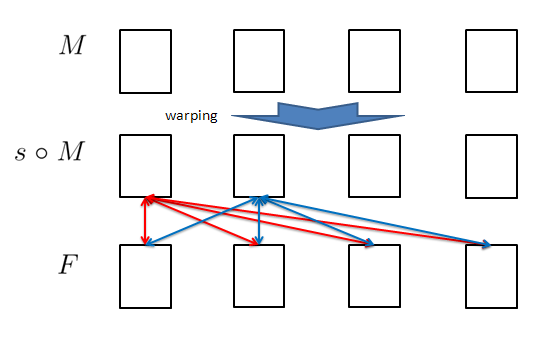
\includegraphics[width=.9\columnwidth]{figs/cross_compare.png}

\end{center}
\caption{Evaluating intergroup registration using cross comparison. Overlapping rates are calculated between every pair of images between the warped moving group and the fixed group.}
\label{fig:cross_compare}
\end{figure}

\subsection{Algorithms and parameters}
	In this section, we briefly describe the compared algorithms, which include the following methods:
	\begin{itemize}
		\item Sharp-mean method. The groupwise registration method in~\cite{Wu20111968} produces a by-product, \ie an adaptively weighted mean image (sharp mean) for each group ($\overline{I}^f$, $\overline{I}^m$ for the fixed and moving groups, respectively). We use the sharp means to represent the image groups, and calculate intergroup transformation $s^{\text{sm}}$ by registering $\overline{I}^f$ and $\overline{I}^m$ using Demons method~\cite{Vercauteren2009S61}.
		
		\item Arithmetic-mean (a-mean) method. This method is essentially the same as the sharp-mean method, except that we use the blurred arithmetic-mean instead of sharp means to represent the groups, and calculate intergroup transformation ($s^{\text{am}}$) accordingly. {\it The arithmetic-mean method serves as a benchmark for comparison}.
		
		\item Histogram-based method. The aforementioned images represent a group of images using weighted or arithmetic means, which are simplistic representations since the intra-group variation is discarded. In contrast, histogram-based method represent a group of images by buildings a histogram field, each voxel of which is a histogram of image intensities. In this preliminary experiment, we build histograms from 35 samples images for each group. The histograms have 128 bins, and intensity values ($[0,255]$) are linearly mapped to the bins using a Gaussian window function of variance equal to 4. The histogram fields are then registered as multi-channel images using the Multi-Channel Demons method in~\cite{peyrat_multichannel_demons}.
	\end{itemize}
	
\section{Results and analysis}

We show preliminary results obtained using two groups of images (AD70 and NC 70). Each group contains 35 subjects, so the results are $35$ by $35$ overlapping rate (Jaccard) matrices. For better visualization, I plotted them using MATLAB {\it imagesc} function. Two types of results are shown here, including the overlapping matrices themselves and the relative comparisons between matrices obtained using different algorithms. 

\subsection{Overlapping matrices}



Figure~\ref{fig:overlapping} shows the overall overlapping-rate (including WM, GM, and VN) matrices. We have the following observations:
\begin{itemize}
	\item Both A-mean and histogram-based methods improve overlapping rates, but A-mean seems to be doing a better job. Nevertheless, the overlapping rate of A-mean method is still very low (less than 35 percent). Overlapping rate of white-matter (WM) alone (Figure~\ref{subfig:wm}) is generally better than the overall overlapping rate (Figure~\ref{subfig:overall}, but is still far from the results reported in the literature~\cite{Wu20111968}.
	\item Sharp-mean method produces spiky results (Figure~\ref{subfig:intergroup_sharpmean}) that favors good alignment between the first subjects of the two groups, but alignments between other subjects are much worse.
\end{itemize}



\begin{figure}[h!!]

\begin{center}
\subfigure[No registration]{
	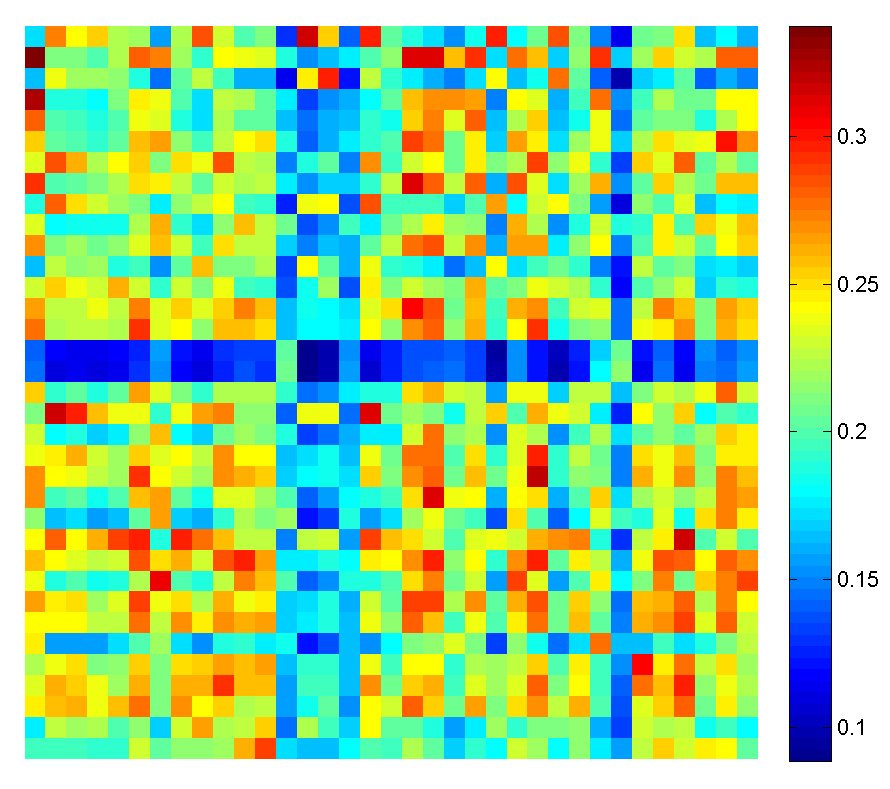
\includegraphics[width=.45\columnwidth]{figs/R_dummy.png}
}
\subfigure[Arithmetic mean]
{
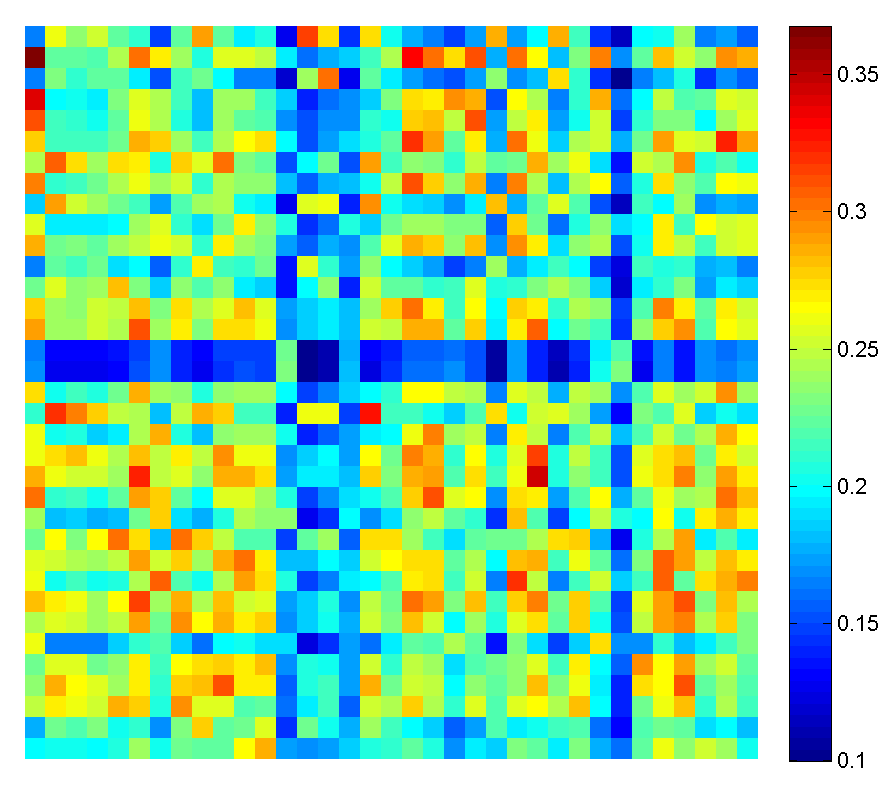
\includegraphics[width=.45\columnwidth]{figs/R_groupmean.png}
}
\\
\subfigure[Sharp mean]
{
	\label{subfig:intergroup_sharpmean}
	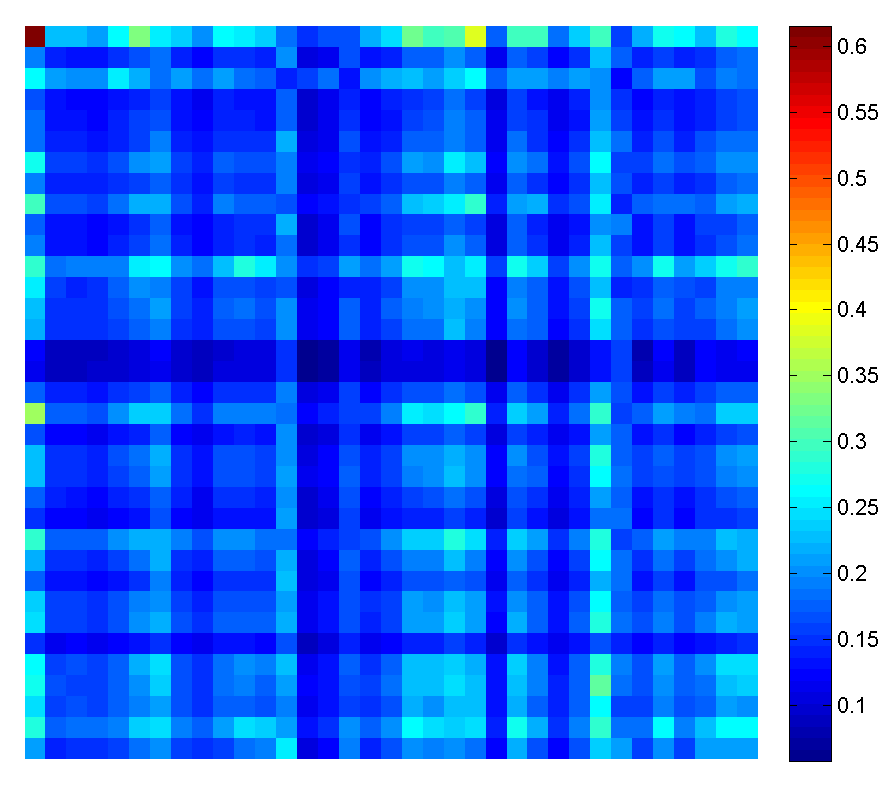
\includegraphics[width=.45\columnwidth]{figs/R_sharpmean.png}
}
\subfigure[Histogram-based]
{
	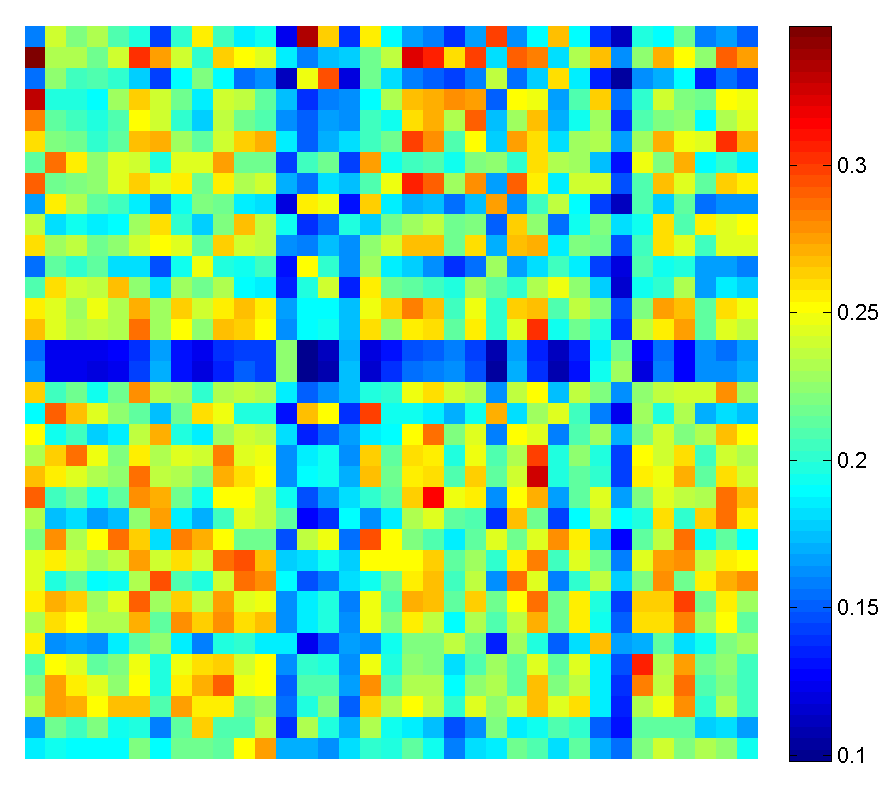
\includegraphics[width=.45\columnwidth]{figs/R_histogram.png}
}

\end{center}
\caption{The overall (regardless WM, GM or VN) overlapping-rate matrices. }
\label{fig:overlapping}
\end{figure}

I believe two factors contribute to these observations. {\it First, the groupwise registration step was not carried out properly, leading to poor intragroup alignment to begin with. As a result, intergroup registration became difficult and produced low overall overlapping rate.} To verify, I first calculated the mutual overlapping rate \emph{within} the moving group. The result happens to be a matrix of the same size as the intergroup overlapping matrix, but measures the quality intragroup alignment. Figure~\ref{fig:groupwise} shows the \emph{groupwise} overlapping matrices for all labels and white-matter (WM). Naturally, the diagonal elements will be one as the images are perfectly aligned to themselves, but the alignment between different images is poor (with overlapping rate less than {\bf 30\%}). Even for white-matter, {\bf the best overlapping rate is around 50 percent only}. {Nevertheless, this problem is not essential, as Guorong has promised to produce better results and I may run his code myself.}



\begin{figure}
\begin{center}
\subfigure[Overall]
{
	\label{subfig:overall}
	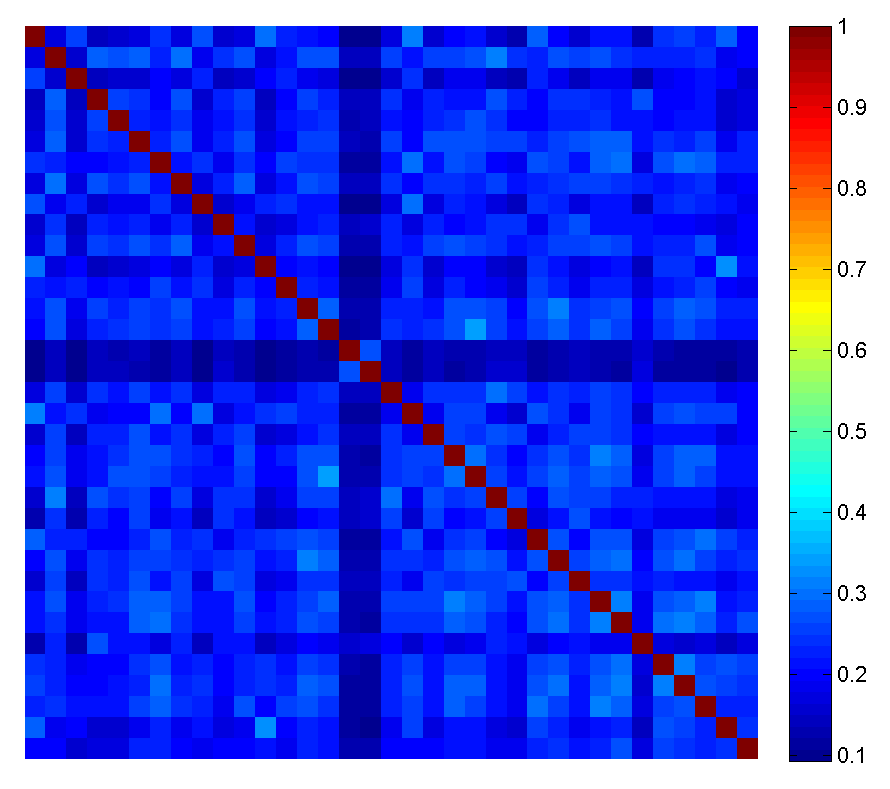
\includegraphics[width=0.45\columnwidth]{figs/R_groupwise.png}
}
\subfigure[WM]
{
	\label{subfig:wm}
	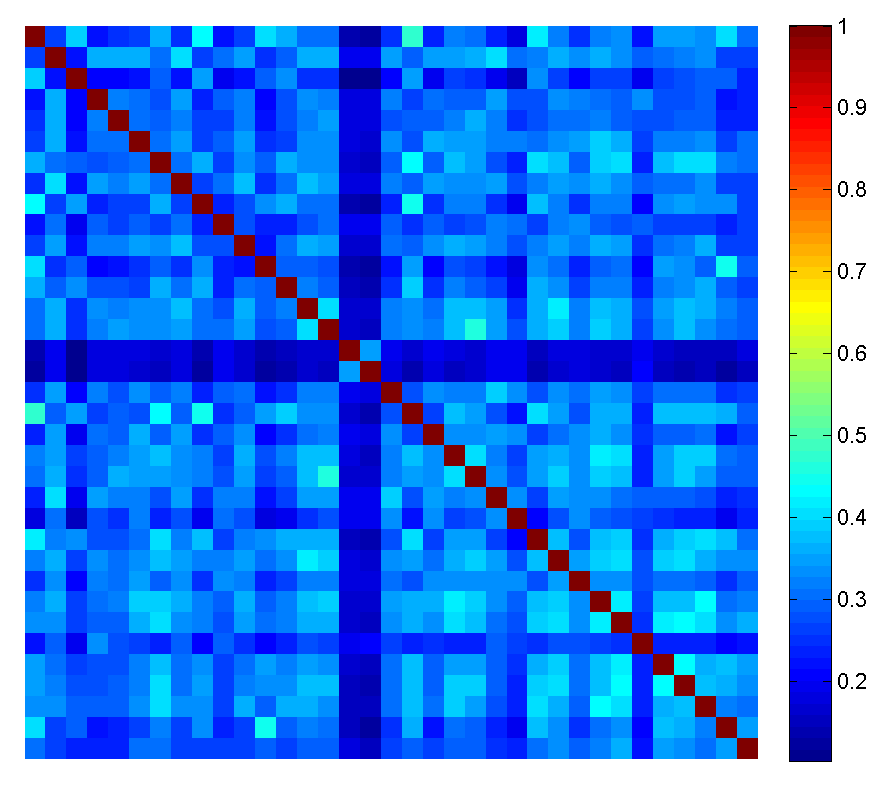
\includegraphics[width=0.45\columnwidth]{figs/wm/R_groupwise.png}
}
\end{center}
\caption{Intragroup mutual overlapping rate of the images in the moving group. Low overlapping rates indicate that the groupwise registration was not carried out properly.}
\label{fig:groupwise}
\end{figure}


{\it Second, sharp-mean produced spiky result probably due to its inheritt bias towards certain heavily-weighted subjects.} This limitation of sharp-mean is more-or-less expected. To verify, I calculated the similarity (sum of squared difference) between the sharp-mean and the subjects in group AD70, using ITK build-in programs. The result distances of first 18 subjects in AD70 (moving group) are shown in Figure~\ref{fig:sharpmean_similarity}. Coincidently, group NC70 (fixed group) shows similar pattern in that the first subject resembles the sharp-mean most. As a result, I believe sharpmean produced best alignment between the first subjects of the two groups. In addition, it is fairly understandable that subject 16 and 17 have the lowest intergroup alignment, since they are most different from the sharp-mean.

\begin{figure}
\begin{center}
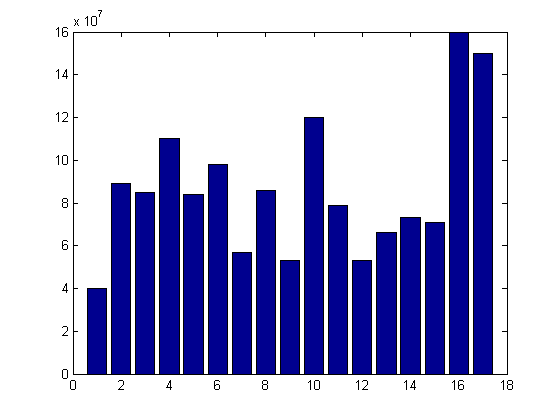
\includegraphics[width=.9\columnwidth]{figs/sharpmean_similarity.png}
\end{center}
\caption{Similarity of sharpmean to the group members.}
\label{fig:sharpmean_similarity}
\end{figure}

The observations described above more-or-less fell in the line I expected. In the following section, I compare these algorithms and study how much benefit we get by using histogram-based registration.

\subsection{Comparison of overlapping matrices}

First, we compare the three algorithms (A-mean, sharp-mean, and histogram-based method) to the overlapping rate $\OverlapMatDummy$ calculated {\bf without intergroup registration}. For intuitive visualization, we subtract their corresponding matrices (\ie, $\OverlapMatMean$,$\OverlapMatSharpMean$,$\OverlapMatHistogram$) by the initial overlapping rate matrix (\ie $\OverlapMatDummy$), and obtain logic matrices indicating the results' positiveness. The positive entries of the difference matrices indicate cases where improvement has been observed. Figure~\ref{fig:relative} shows plotted logic matrices. It is clear that A-mean improved intergroup alignment on most cases, while sharp-mean actually make most cases worse. Histogram-based method improves alignment in {\bf 51\%} of the cases (85\% for A-mean). The improvement of histogram-based registration seems marginal. To further verify, I simply calculated total Jaccard overlapping rates $\sum \OverlapMatHistogram$  and $\sum \OverlapMatDummy$. The improvement of former regarding to the latter is only {\bf 1} percent (8 percent for A-mean).

\begin{figure}
\subfigure[Sharp-mean]
{
	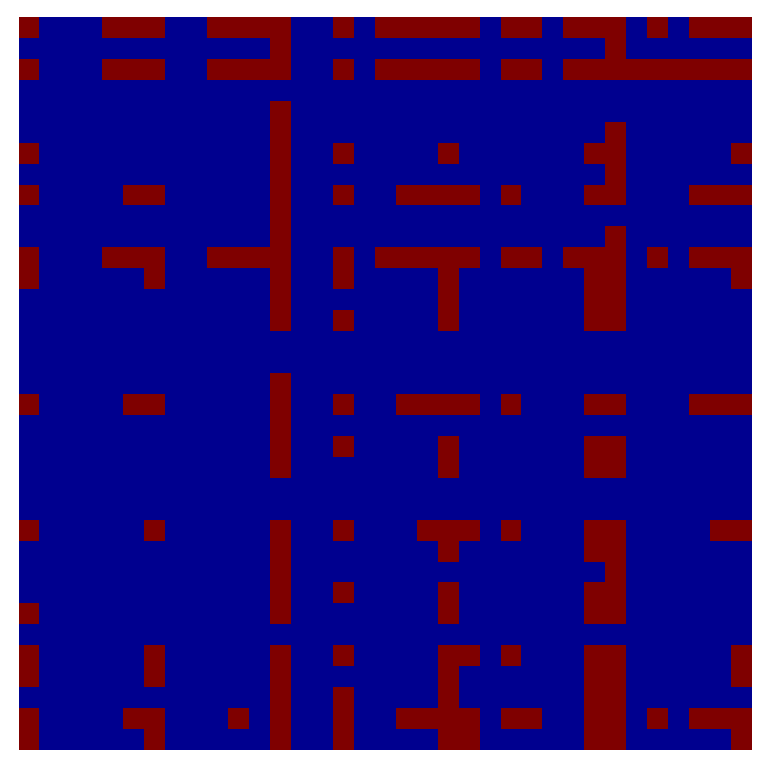
\includegraphics[width=0.3\columnwidth]{./figs/log_sharpmean.png}
}
\subfigure[Histogram-based]
{
	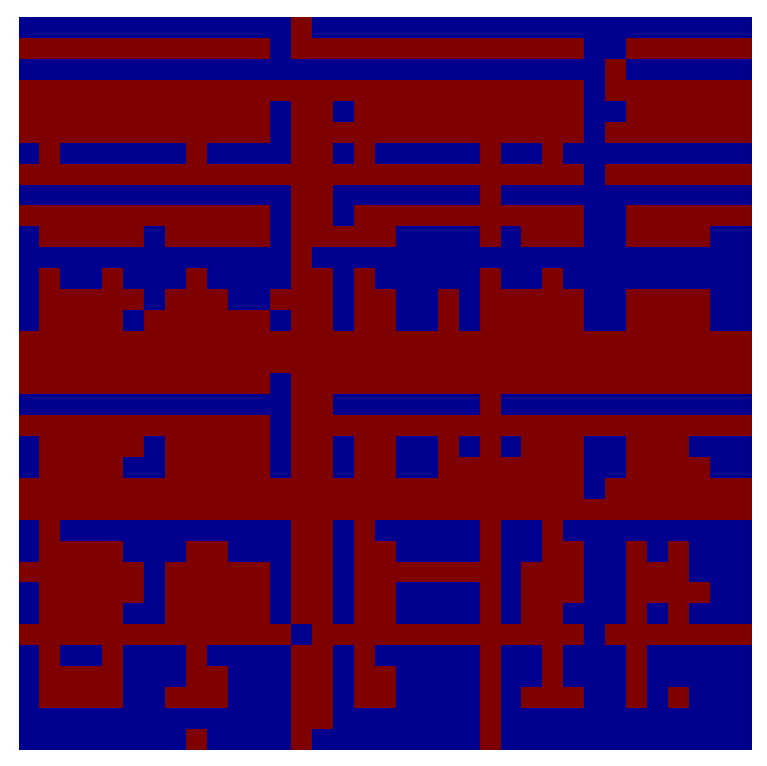
\includegraphics[width=0.3\columnwidth]{./figs/log_histogram.png}
}
\subfigure[A-mean]
{
	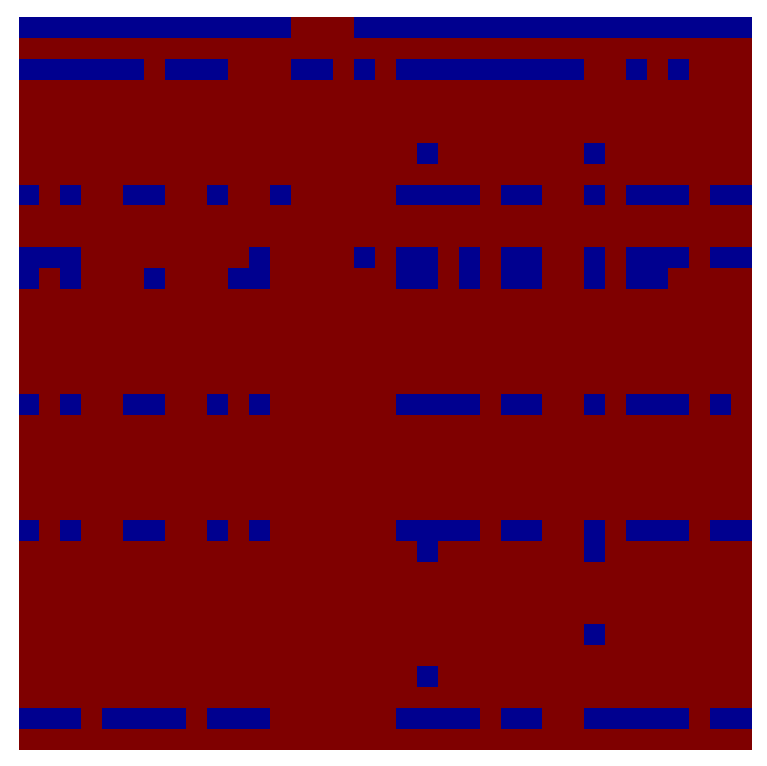
\includegraphics[width=0.3\columnwidth]{./figs/log_groupmean.png}
}
\caption{Cases where intergroup registration improved overlapping rate. Brown boxes indicates improved cases.}
\label{fig:relative}
\end{figure}

\subsection{Why histogram-based method performed poorly}
Here I theoretically show the relation between histogram-based method and A-mean, and discuss why simple histogram-based method may not outperform A-mean, and what can be done to improve it.

\subsubsection{A-mean is another histogram-based method}
It turns out that A-mean is closely related to histogram-based method. In our current histogram-based method, we used simple Euclidean distance measure for registration. If we represent a histogram as a vector $P=\left\{ p_1, p_2, \cdots, p_\NBin \right\}^\Transpose$, where $\NBin$ is the number of bins, then the distance between two histograms is given by the squared-root of the following:
\begin{align}
L^2(P_1,P_2)=(P_1-P_2)^\Transpose(P_1-P_2).
\label{eq:histogram_distance}
\end{align}
A more sophisticated distance measure is based on Jensen-Shannon divergence, but we will discuss later that J-S divergence might also suffer from similar limitations.

On the other hand, the mean values are defined as:
\begin{align}
m(P_1)=\sum_i f_i p_i=P_1^{\Transpose} F,
\end{align}
where $f_i$ are the intensity values (\eg $0,1,\ldots,255$). When we register mean images using Demons algorithm, we are essentially calculating the SSD error as follows:
\begin{align}
SSD(m_1,m_2)&=(m_1-m_2)^2 \notag \\
						&=\left((P_1^\Transpose-P_2^\Transpose) F\right)^2 \notag \\
						&=(P_1-P_2)^\Transpose \underbrace{F F^\Transpose}_{\text{the kernel}} (P_1-P_2).
\label{eq:mean_distance}
\end{align}

Comparing the distance measure using mean values (Equation~\ref{eq:mean_distance}) and histogram-based distance (Equation~\ref{eq:histogram_distance}). It is clear that the kernel matrix $F F^\Transpose$ is missing in histogram-based distance.

It is clear that $F F^\Transpose$ puts more importance on the histogram bins corresponding high-intensity values (a 0.1 variation in the probability of white matter has more influence in SSD than the same amount of variation in VN). Table~\ref{tb:percentage} shows the percentage of improved cases regarding to three types of labels (WM, GM, VN). It is clear that A-mean's performance increases sharply with intensities of the labels, while histogram-based method is pretty much stable. Histogram-based method still increases slowly with the intensities. However, I believe it is because that the WM has lower variance in their histograms and thus still results in better alignment.
This is natural since high-intensity values do carry more information. This also falls in line with the rules that mean values is often used to minimize sum-of-squared-differences (SSD). \emph{By using histograms only, we are only using the distribution of the random signal, but ignored the meaning of the signal itself}. 

Histogram-based registration works in a similar way as mutual information, and I will further investigate. Meanwhile, I suspect J-S divergence would not significantly improve histogram-based method by itself. Furthermore, I believe sharp-mean can be similarly interpreted as a histogram-based method using adaptive kernel matrices.
Despite these setbacks, there is still a bright side of the story as will be discussed in the following section.
\begin{table}[thb]
	\caption{Percentage of improved cases}
	\begin{center}
		\label{tb:percentage}
		\begin{tabular*}{0.90\textwidth}{@{\extracolsep{\fill}}cccc}
			%\caption{Average Angular Error}
			\toprule
			Method 	& VN & GM & WM \\
			\midrule
			A-mean  & 56\% & 66\% & 86\% \\
			Histogram & 45\% & 56\%   &58\% \\
			\bottomrule
		\end{tabular*}	
	\end{center}
\end{table}


\subsection{Ways to diagnosis and improve}

First, I may verify the analysis above by adapting the current histogram-based method using a kernel matrix $F F^\Transpose$ to see if it does produce similar results to the A-mean method. If so, I may combine histogram-based method with A-mean, since they have the same histogram-based framework. A parameter can be adopted to control the weight of histogram-based distance measure.
{\it More importantly, we may replace $F F^\Transpose$ with an kernel matrix optimally trained according to the registration results.} This way, we essentially learn a similarity metric for intergroup registration, and the kernel matrix may even vary spatially.


\section{Intergroup registration based on Mahalanobis distance}
\label{sec:mahalanobis}
As we have previously found out that histogram-based intergroup registration method performed poorly in comparison to mean-based method, mainly because that histogram-based method only compares the distributions of image intensities but ignores the information carried by the intensity values. To improve, we propose to use Mahalanobis distance that combines the mean and variance of a group of images. {\bf Preliminary results of the proposed method show subtle improvement over mean-based method.}

\subsection{General idea}
Mean-based intergroup registration use simple Euclidean distance (Equation~\ref{eq:mean_distance}) to measure image dissimilarity, while ignoring intragroup variations. We amend Equation~\ref{eq:mean_distance} by including the variance parameter using Mahalanobis distance, defined as:
\begin{align}
MAH(m_1,m_2)=\frac{(m_1-m_2)^2}{\sigma^2_1}.
\end{align}
Here, $\sigma_1$ is the voxel-wise variance estimated from the moving group samples. Similarly to the symmetric Demons algorithm, a symmetric Mahalanobis distance is used in my implementation, given by:
\begin{align}
MAH(m_1,m_2)=\frac{(m_1-m_2)^2}{\sigma^2_1}+\frac{(m_1-m_2)^2}{\sigma^2_2},
\label{eq:symmetric_mahalanobis}
\end{align}
with variance $\sigma_2$ estimated from the fixed group samples. At some voxels (\eg the background), image variance can be zero, causing numerical problems. As a result, a parameter $\sigma_0>0$ is chosen so that {\bf  the estimated sample variance is trunked to $\sigma_0$ from below}. Derivation of the equations for Demons algorithm is straight-forward and thus is omitted here.

Presumably, the inclusion of image variance reduce the influence of image regions with large intragroup variations. In other words, {\it if the group member do not agree in some regions, then these places will be given less emphasis for intergroup registration}. Hopefully, this would allow better handling of uncertainties and outliers.

\subsection{Preliminary results}
The setup of this experiment is the same as our previous ones (Section~\ref{sec:introduction}), but here we only compare mean-based registration method (A-mean) and the proposed method (Mah-Demons), since A-mean previously produced the best results. It is worth pointing out that both methods use the same parameters for smoothing the vector fields. The only difference is that Mah-Demons has an extra parameter $\sigma_0$ for truncating the sample variations from below. We set $\sigma_0=1$ by default. 
Figure~\ref{fig:relative_mah} shows the relative improvement of Mah-Demons over A-mean represented as a 35 by 35 relative difference matrix, whose elements are calculated as follows:
\begin{align}
R^{\text{improve}}=\frac{\OverlapMatMah-\OverlapMatMean}{\OverlapMatMean},
\end{align}
where $\OverlapMatMah$ and $\OverlapMatMean$ are the cross-comparison overlapping matrices of Mah-Demons and A-mean methods, respectively.
The improvement of overlapping rate on one best case is 1.5 percent, while the average improvement on $35\times 35$ cases is 0.04 percent, which is still quite small. The good news is that Mah-Demons did not perform worse than A-mean at least.

\begin{figure}[h!!!!!!!!!!!!tb]
\begin{center}
	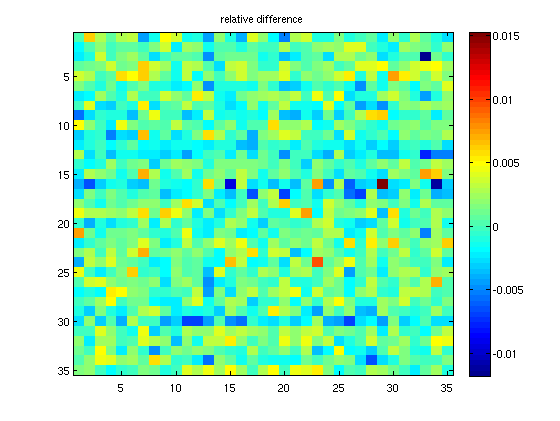
\includegraphics[width=.8\linewidth]{figs/relative_improvement.png}
\end{center}

\caption{Relative improvement of Mah-Demons over mean-based method. Maximally, 1.5 percent of improvement can be observed in one case.}
\label{fig:relative_mah}
\end{figure}

Figure~\ref{fig:cases_mah} shows the cases where positive improvements can be observed. {\bf 57 percent} of the cases from a total of $35\times 35$ were improved, which can be said as a small majority.

\begin{figure}[h!!!!!!!!!!!!tb]
\begin{center}
	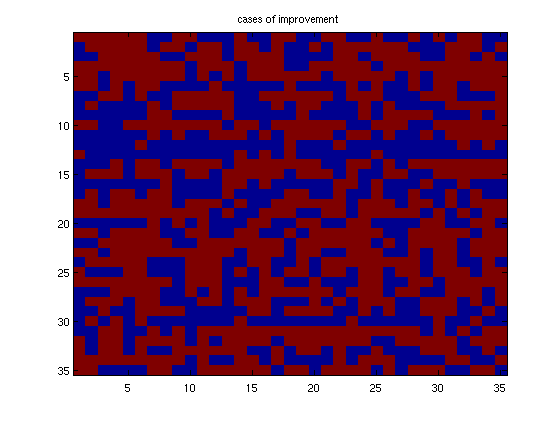
\includegraphics[width=.8\linewidth]{figs/cases_improved.png}
\end{center}

\caption{Cases where improvements have been observed (brown boxes indicates an improvement in the overlapping rate). {\bf 57\%} of the cases were improved.}
\label{fig:cases_mah}
\end{figure}

\subsection{Future work}
Given the preliminary nature of this work, there are still many investigations to be made. Here, I sketchily list a few.

\begin{itemize}
	\item Tuning parameters. So far, the image background always has the lowest variation, which give them undesired priority in registration. I believe this problem could be lessened by assuming some kind of background uncertainty level. Also, the Mahalanobis distance also changed the relative weighting of smoothing factor, so more extensive parameter tuning might further improve the results.
	\item Testing on a larger group of images with possibly more outliers. The proposed method is supposedly better at handling outliers and intragroup variations. I need a few examples to show this is the case.
	\item Mahalanobis distance is closely related to Gaussian distribution. A probability framework may be derived for this method, and better distribution representation could be adopted. However, this only makes sense when we have more substantial improvements.
\end{itemize}

\section{Improved Mah-Demons method}
\label{sec:improved}
In this section, I describe the improvements following the work described in previous section (Section~\ref{sec:mahalanobis}), mainly in two aspects: methodology and data. For methodology, I adopted a background variance parameter that better reflects uncertainties in the background regions. Secondly, I used gradient-descent method for tuning the parameters. {\bf These adaptations indeed improved the results, but the improvements are still not significant}. Alternatively, I used an updated dataset from Guorong.  {\bf On this new dataset, improvement of Mah-Demons over mean-based registration method is greater.} Finally, I did some analysis and diagnosis. {\bf I suspect there are several approaches to further improve the method,  but have not been able to make conclusions yet.}

\subsection{Incorporation of background variance parameter}
The key idea of background variance parameter is that in background areas, the data variance is usually very low, due to lack of information rather than high consistency in the sample data. The Mahalanobis distance in background regions (Equation~\ref{eq:symmetric_mahalanobis}) will be skewed due to the low variance, and making it sensitive to background image noise. Although I capped the variance from below using $\sigma_0$ to avoid numerical singularity, this capping does not differentiate between foreground areas with truly low variance and background regions without intensity values. To improve, I used a threshold $\lambda_{bg}$ to segment the background region, and simply set the variance to $\sigma_{bg} >0$ for voxels whose intensity values fall below the threshold $\lambda_{bg}$. $\lambda_{bg}$ is empirically set to 5, as I observed that $\lambda_{bg}=5$ is enough to separate the background regions from ventricle areas.

The percentage of improved cases increases from {\bf 57\% to 61\% }. Average improvement in the overlapping rate increases from {\bf 0.04 percent to 0.1 percent}. Nevertheless, the improved results are still not very impressive. Furthermore, I used gradient-descent to tune the background variance parameter. However, experiments show that the gradient-descent method can easily get stuck in local minima, unable to find an optimal parameter. I manually restart the search with a number of initial values, and found the background variance $\sigma_{bg}=10$ performed reasonably well.

\subsection{Experiments using updated dataset}
The updated dataset is much smaller, containing only 10 subjects for AD70 and NC70 respectively. According to Guorong, the updated datasets are better aligned groupwise, since he was able to run more registration iterations on this smaller dataset. The cross comparison overlapping matrix in this case is of size $10 \times 10$. On this dataset, {\bf 74 \%} percent of the comparison cases were improved. Figure~\ref{fig:cases_mah_updated} shows the improved cases. Figure~\ref{fig:relative_updated} shows the relative differences. On the best case, the overlapping is relatively improved by {\bf 2.5 percent}, and {\bf about 0.5 percent} on average.

\begin{figure}[h!!!!!!!!!!!!tb]
\begin{center}
	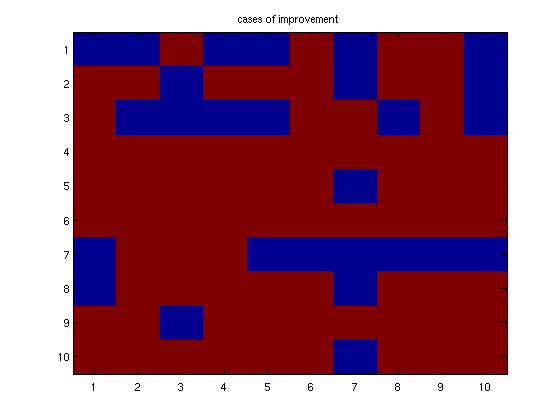
\includegraphics[width=.8\linewidth]{figs/cases_improved2.png}
\end{center}
\caption{Improved cases on the updated dataset.}
\label{fig:cases_mah_updated}
\end{figure}

\begin{figure}[h!!!!!!!!!!!!tb]
\begin{center}
	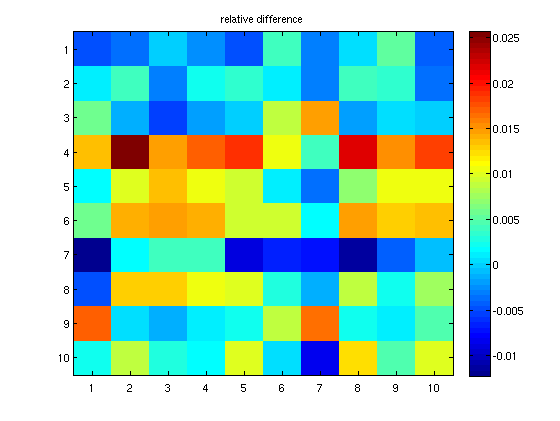
\includegraphics[width=.8\linewidth]{figs/relative_improvement2.png}
\end{center}
\caption{Relative improvement of overlapping rates.}
\label{fig:relative_updated}
\end{figure}

\subsection{Analysis of the results}
As we have seen, the improvements seem to be consistent in both experiments, but the numbers appear to be small. To diagnose, I try to find out where the improvements are, and whether the improvements are related to certain characteristics of the input data. Specifically, I did some analysis on the obtained deformation fields, sample variance, and skewness. On the other hand, I want to find out how significant the improvement can be, \ie whether there is an upper-bound on the improvement of overlapping rates. Accordingly, I am planning on a few more tests. {\it At this point, I am unable to make decisive conclusions.} In the following section, I mainly discuss the observations, and my initial guess to the reasons that cause these observations.

\subsubsection{Difference between Mah-Demons and mean-based method is localized}

Let us begin by denoting the deformation fields as $D_{Mah}$ and $D_{amean}$, produced by Mah-Demons and mean-based intergroup registration, respectively. The difference between these two vector fields result in a third vector field $D_{diff}=D_{mah}-D_{amean}$, and its magnitude $\|D_{diff}\|$ is a scalar field. By examining it visually, we can notice that  $\|D_{diff}\|$ has very large values in relatively small areas and small values elsewhere. Figure~\ref{fig:deform_difference} shows the sagittal section of  $\|D_{diff}\|$. I suspected that $\|D_{diff}\|$ should be related to the sample variance, but immediate examination of sagittal sections of variance maps (Figure~\ref{fig:group_var}) does not provide very strong correlation between the two. I need to better understand this difference and maybe provide some solid and intuitive examples where Mah-Demons can outperform mean-based method.

\begin{figure}[h!!!!!!!!!!!!tb]
\begin{center}
	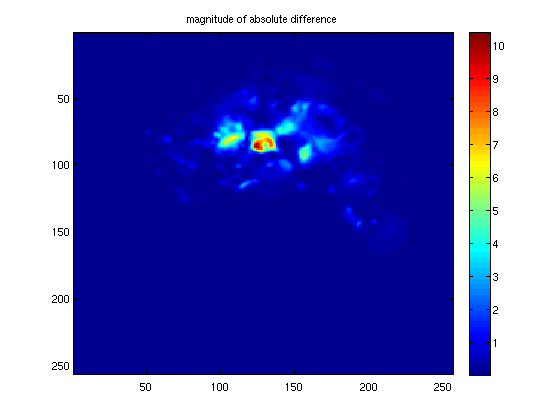
\includegraphics[width=.8\linewidth]{figs/deform_diff.png}
\end{center}
\caption{Magnitude of difference ($\|D_{diff}\|$) between deformation fields obtained by Mah-Demons and mean-based registration.}
\label{fig:deform_difference}
\end{figure}


\begin{figure}[h!!!!!!!!!!!!tb]
\begin{center}
	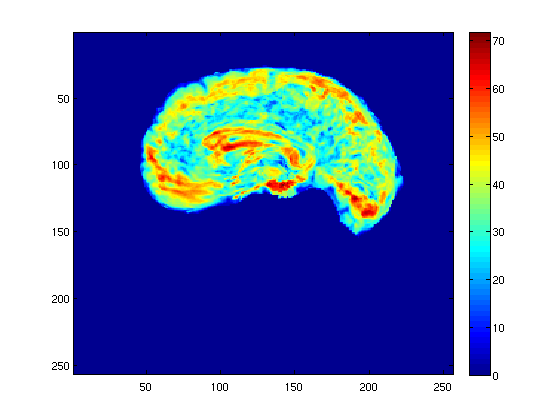
\includegraphics[width=.45\linewidth]{figs/fixed_var.png}
	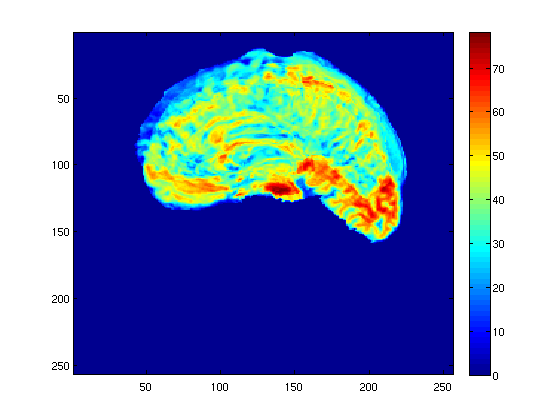
\includegraphics[width=.45\linewidth]{figs/moving_var.png}
\end{center}
\caption{Sample variations in each group (left: AD70, right: NC 70). It is not very obvious that $\|D_{diff}\|$ is related to the variance maps. }
\label{fig:group_var}
\end{figure}



\subsubsection{Is variance alone enough to describe the sample data?}
Mahalanobis distance is related to Gaussian model, and can be interpreted as a maximum likelihood formulation. A key assumption is that sample data is normally distributed. To verify, I calculated the skewness of the obtained histograms. Figure~\ref{fig:skewness} shows a section of the skewness map. It is clear that sample distribution along the boundary can be seriously skewed. Figure~\ref{fig:skewness_index} shows a number of distributions (histograms) with different skewness index. It is clear that  highly-skewed distributions may be multi-modeled (distribution in the center), with some areas contain significant amount of background voxels (distribution on the right).
Ideally, normal distributions have zero skewness (perfect symmetry). Higher skewness indicates severe violation of the Gaussian distribution assumption. As a result, these voxels might cause problem for the Mah-Demons method. More sophisticated probability model may improve the result, but I am not sure how much improvement we can get out of it.

\begin{figure}[h!!!!!!!!!!!!tb]
\begin{center}
	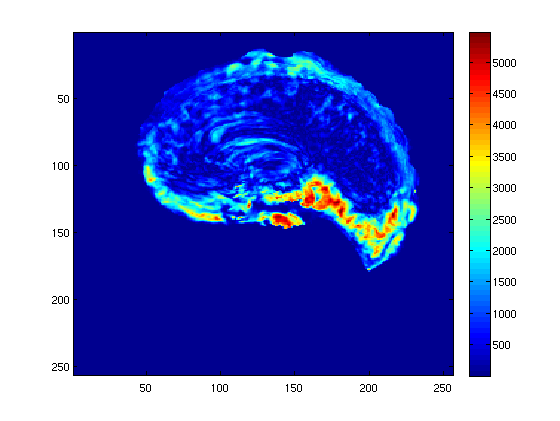
\includegraphics[width=.8\linewidth]{figs/skewness.png}
\end{center}
\caption{Skewness of sample distribution. Note that regions of high variance not necessarily have high skewness.}
\label{fig:skewness}
\end{figure}

\begin{figure}[h!!!!!!!!!!!!tb]
\begin{center}
	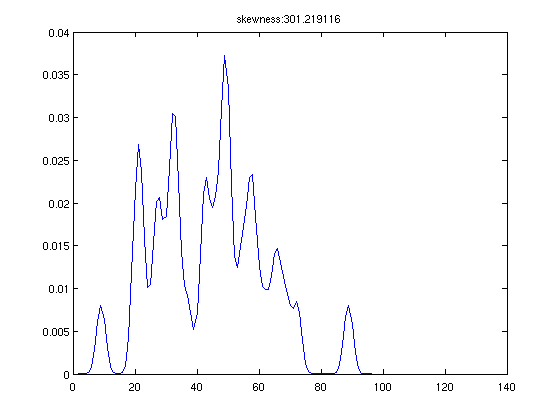
\includegraphics[width=.3\linewidth]{figs/skewed_300.png}
	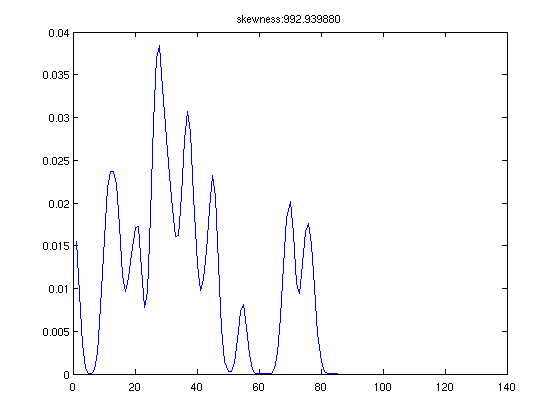
\includegraphics[width=.3\linewidth]{figs/skewed_1000.png}
	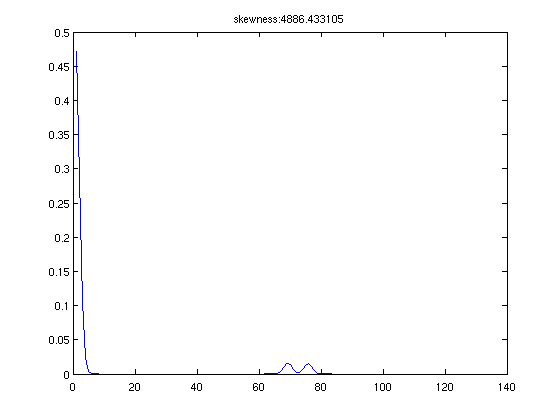
\includegraphics[width=.3\linewidth]{figs/skewed_4886.png}
\end{center}
\caption{Distributions of different skewness index (from left to right: 300,1000,4886). Highly skewed histograms may not be well modeled by Gaussian functions. {\bf The Parzen window size is not properly set, so the histograms are not smooth, but their relative skewness is not affected. }}
\label{fig:skewness_index}
\end{figure}

\subsubsection{How much improvement is possible in the overlapping rate?}
In other words, is there an {\bf upper-bound} on the improvement of overlapping rate using intergroup registration? I believe we can get a good estimate of that by combing the two groups into one, and run a groupwise registration algorithm on the combined group. After groupwise alignment, we can still calculate the cross comparison overlapping rate matrix. If the upper-bound itself shows only small improvement over mean-based intergroup registration, then our previously mentioned  improvement of Mah-Demons may be {\bf relatively significant}.
I suspect that if the two groups are not very different from each other, then groupwise registration on individual groups or the combined group will not be very different either. 

At last, even though the overlapping rate is only slightly improved, these improvements may happen in some important regions. Its significance might still be justified if evaluation shows that Mah-Demons improves the accuracy of some higher-level applications, such as segmentation and classifications.

\FloatBarrier

{\small 
\bibliographystyle{unsrt}
\bibliography{wei_intergroup}
}



\end{document}

\endinput
%%
%% End of file `elsarticle-template-num.tex'.









